\documentclass[conference]{IEEEtran}
\usepackage{times}
\usepackage[numbers]{natbib}
\usepackage{amsmath,amssymb,graphicx,booktabs,tabularx,flushend}
\usepackage[bookmarks=true,hidelinks]{hyperref}
\hypersetup{pdftitle={When Does Reading a Cartesian Target Change Robot Replay?},pdfauthor={},pdfsubject={Cartesian control and demonstration replay}}
\newcommand{\clip}{\operatorname{clip}}
\newcommand{\dist}{\operatorname{dist}}
\newcommand{\vect}[1]{\boldsymbol{#1}}
\begin{document}


\title{When Does Reading a Cartesian Target Change Robot Replay?}

\author{Author Names Omitted for Anonymous Review}

\maketitle

\thispagestyle{empty}\pagestyle{empty}

\begin{abstract}

During demonstration replay, a robot can typically measure its end-effector position, whereas the Cartesian target stored internally by the controller may remain hidden. This paper derives how much reading back that internal target reduces worst-case error under single-step command limits, and then examines how the resulting target shift propagates to physical contact and task outcomes. In a simulated Panda lifting task, a single readback corrects an average command-origin estimation error of $120.32\,\text{mm}$; however, because the upward displacement command is already saturated, the next written target changes by only $0.026\,\text{mm}$ on average. Across 216 paired Sawyer pushing comparisons spanning 24 layouts, every pair differs in its written target by at least $1\,\text{mm}$, and 105 pairs exhibit a measurable change in first contact; readback rescues 6 pushes while causing 12 otherwise successful pushes to fail. Across another 24 layouts (144 test conditions), a state-based policy that schedules readbacks from end-effector motion and command history issues 76 queries and succeeds on the exact same 75 conditions as a no-readback observer. Single-step geometric computation reliably identifies when acquiring the hidden target helps correct the command, yet whether that correction improves physical manipulation still depends on how the end-effector makes contact with the object.

\end{abstract}

\IEEEpeerreviewmaketitle

\section{Introduction}

In a simulated Panda lifting rollout, the replay controller's estimate of the next command origin drifts by approximately $120\,\text{mm}$. Because both compared branches already request the maximum upward displacement at that step, reading back the true origin shifts the next written target by an average of only $0.026\,\text{mm}$. Four control steps later, however, the mean written targets of the two branches diverge by $53.82\,\text{mm}$ (Fig.~\ref{fig:mechanism}). By contrast, during the descent phase, although the initial origin estimation error is smaller, readback shifts the written target by an average of $24.13\,\text{mm}$, yet both branches ultimately lift the block. This contrast raises a central question: under what conditions does reading the controller's internal Cartesian target actually alter task outcomes?

A Cartesian displacement command can be executed either relative to the currently measured end-effector position or relative to the previous target stored by the controller. In the latter mode, if the receiver zeroes out an input without notifying the sender, integrating the sent command history reconstructs an erroneous reference origin. The replay policy must then either infer the target from observed end-effector motion or query the controller directly for a readback.

\begin{figure}[t]
\centering
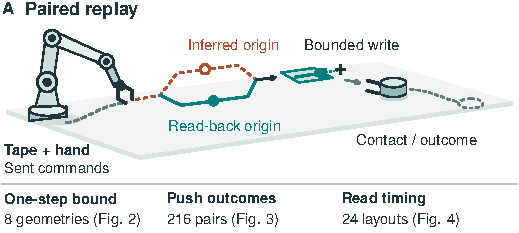
\includegraphics[width=\columnwidth]{figures/study-workflow.pdf}\par
\makebox[\columnwidth][l]{\small\textsf{\textbf{B\quad Panda measurements}}}\par
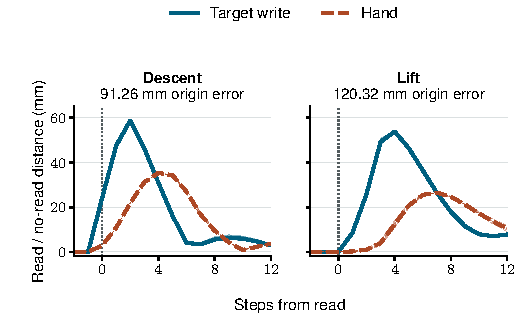
\includegraphics[trim=0 6bp 0 0,clip,width=\columnwidth]{figures/origin-readback.pdf}
\caption{(A) Two replay branches operate on the same source demonstration by either estimating or reading back the command origin before issuing bounded displacement commands. (See Section IV-F and Fig.~\ref{fig:contact} for Sawyer object trajectories, final frames of both branches, and all paired outcomes.) (B) Divergence between the two branches in written target and end-effector position during Panda descent and lifting. Time zero marks the readback step; thin lines show 8 individual layouts, thick lines show the mean, and labels above denote the mean origin estimation error prior to readback.}
\label{fig:mechanism}
\end{figure}

Our central hypothesis is that a single readback improves the next target write only when distinct candidate origins call for different feasible corrections. Action saturation can limit the effect of a read on the next write; Section~III gives the precise condition under which a read leaves the worst-case target loss unchanged. An origin estimate derived from end-effector measurements can also make the worst-case benefit zero. Furthermore, to alter the outcome of a contact-rich task such as pushing, the difference in written targets must also physically affect the manipulated object.

\section{What Is Observable During Replay}

Prior work on action spaces has shown that a robot's low-level control interface substantially shapes learned manipulation behavior \citep{ref1}. For instance, ManiSkill2 converts demonstrations between different action spaces, including controllers referenced to measured poses versus target poses \citep{ref2}, while MimicGen maps end-effector target poses into bounded robot actions \citep{ref3}. Here, we study a controller receiving demonstration commands whose current reference origin may remain hidden to the sender even when the source demonstration and action conventions are known. Under this setting, we evaluate the marginal information gained by directly reading back that reference position.

From a networked control perspective, event-triggered control schedules communication based on state measurements \citep{ref6}, and execution acknowledgments eliminate uncertainty over which inputs actually reached the plant \citep{ref5}. The readback message considered in this work specifically reports the Cartesian target stored inside the controller. Starting from the next target write, we trace how this message cascades through end-effector motion and object contact.

Let $\mathbf{x}_t^\star$ and $\mathbf{x}_t$ denote the end-effector positions immediately before the $t$-th command in the source demonstration and during replay, respectively (superscript $\star$ denotes source-demonstration quantities), and let $\mathbf{g}_t^\star$ be the target written by the $t$-th command in the source demonstration. A readback returns the target currently stored on the receiver. Given the current command's displacement origin $\mathbf{b}$ and commanded displacement $\mathbf{d}$ (both in meters), the controller writes:

\begin{equation}
F(\mathbf{b},\mathbf{d}) = C(\mathbf{b} + \mathbf{d}), \quad \mathbf{d} \in \mathcal{D} = [-\mathbf{s}, \mathbf{s}].
\label{eq:e1}
\end{equation}

Here, $\mathbf{s}$ is a vector of nonnegative per-axis displacement limits, $C$ clips each coordinate to its workspace interval, and vector intervals denote Cartesian products of per-axis intervals. A measured-origin controller sets $\mathbf{b} = \mathbf{x}_t$, whereas an accumulated-origin controller sets $\mathbf{b}$ to the target actually written at the previous step. In accumulated mode, once an input is overwritten or dropped, the same history of sent actions can be consistent with two different origins; only as the controlled arm responds physically does subsequent end-effector motion reveal the discrepancy.

\section{How Much Can One Readback Help?}\label{sec:theory}

We first analyze a single update step. Suppose the true origin $\mathbf{b}$ lies within a known box $\mathcal{B} = [\mathbf{L}, \mathbf{H}]$, the desired target is $\mathbf{h}$, and the next command will reach the target-writing function intact, with an option to read the true origin beforehand. Define the per-step squared target error $\ell(\mathbf{b}, \mathbf{d}) = \Vert{} F(\mathbf{b}, \mathbf{d}) - \mathbf{h} \Vert{}_2^2$. Without and with readback, the achievable worst-case (minimax) losses are:

\begin{equation}
\begin{aligned}
V_0 &= \min_{\mathbf{d} \in \mathcal{D}} \max_{\mathbf{b} \in \mathcal{B}} \ell(\mathbf{b}, \mathbf{d}), \\
V_1 &= \max_{\mathbf{b} \in \mathcal{B}} \min_{\mathbf{d} \in \mathcal{D}} \ell(\mathbf{b}, \mathbf{d}).
\end{aligned}
\label{eq:e2}
\end{equation}

Without readback, a single displacement $\mathbf{d}$ must serve all candidate origins in $\mathcal{B}$. With readback, the replay policy can tailor $\mathbf{d}$ to the observed origin. The gap $V_0 - V_1$ (in $\text{m}^2$) measures the exact reduction in worst-case squared target error afforded by one readback.

\textbf{Closed-form computation.} Fix a coordinate axis and let $b, d, h, L, H, s$ denote the corresponding scalars, keeping $C$ for the per-axis workspace clip. Given $b$, the reachable target interval is $I_b = [C(b - s), C(b + s)]$, whose endpoints vary monotonically with $b$. Consequently, the worst-case distance from $h$ to $I_b$ is:

\[
r_1 = \max\{\operatorname{dist}(h, I_L),\, \operatorname{dist}(h, I_H)\}.
\]

If a single displacement $d$ is issued for all candidate origins, the worst-case absolute error is:

\[
r(d) = \max\{h - C(L + d),\, C(H + d) - h\}.
\]

As $d$ increases, the first term is nonincreasing and the second term is nondecreasing. If the two terms intersect within $[-s, s]$, their intersection minimizes $r(d)$; otherwise, the optimum lies at one of the action-interval endpoints. Because both terms are piecewise affine, minimizing $r(d)$ only requires evaluating the two action endpoints, the workspace-clipping breakpoints, and any intersections between adjacent breakpoints. The per-axis losses are thus $v_0 = \min_{-s \le d \le s} r(d)^2$ and $v_1 = r_1^2$. Readback strictly reduces the worst-case loss on that axis if and only if no common displacement $d \in [-s, s]$ satisfies both

\begin{equation}
C(L + d) \ge h - r_1, \quad C(H + d) \le h + r_1.
\label{eq:e3}
\end{equation}

Since both $\mathcal{D}$ and $\mathcal{B}$ are Cartesian products and the squared Euclidean loss is additive across axes, $V_k = \sum_{j=1}^3 v_{k,j}$ for $k \in \{0, 1\}$. Note that replacing a non-axis-aligned uncertainty set with an enclosing bounding box ignores cross-axis correlations and alters the modeled uncertainty.

\begin{figure}[t]
\centering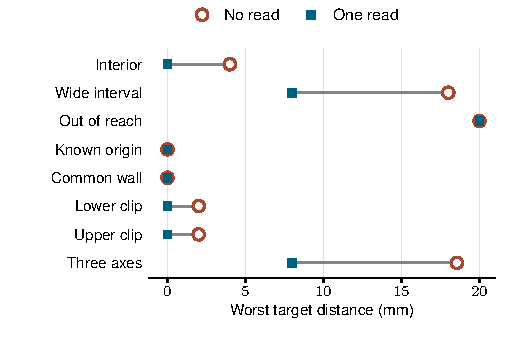
\includegraphics[trim=0 11bp 0 0,clip,width=\columnwidth]{figures/one-step-geometry.pdf}
\caption{Worst-case Euclidean target distance (in $\text{mm}$) across eight predefined geometric conditions when using a single shared command versus origin-specific commands. Points are computed from Sawyer's native target-writing function across two tasks and two random seeds per task, which coincide exactly. Overlapping symbols on a row indicate that reading the origin does not reduce the worst-case loss under that condition.}
\label{fig:geometry}
\end{figure}

We evaluated Sawyer's native target-writing function 1,088 times---probing 17 origins (including all box vertices) per geometry, task, seed, and readback setting. Across every geometric condition, the observed maximum squared errors matched the two analytical losses exactly (Fig.~\ref{fig:geometry}). When the candidate origin interval is wide, readback lowers the worst-case distance from $18\,\text{mm}$ to $8\,\text{mm}$; when no reachable target can attain the desired position, the worst-case distance remains $20\,\text{mm}$ either way. Even when the worst-case losses are equal, readback can still improve performance at specific realized origins.

\section{Paired Replay Experiments}

\subsection{Preserving Motion from Demonstrations}

For each scripted source demonstration, we record end-effector positions, control targets, command scales, and gripper timing. All compared policies share the exact same initial state and perturbation schedule. The \textbf{direct-copy} policy simply resends the recorded actions open-loop. Under the \textbf{target-reconstruction} policy, the desired target to write is defined via end-effector feedback:

\begin{equation}
\mathbf{h}_t = \mathbf{g}_t^\star + k(\mathbf{x}_t^\star - \mathbf{x}_t),
\label{eq:e4}
\end{equation}

where $k$ is the end-effector position feedback gain. When the replay end-effector position matches the demonstration, $\mathbf{h}_t$ reduces to $\mathbf{g}_t^\star$. Given an origin estimate $\widehat{\mathbf{b}}_t$, the replay policy retains the demonstrated displacement if applying it from $\widehat{\mathbf{b}}_t$ writes $\mathbf{h}_t$; otherwise, it sends the clipped correction:

\[
\mathbf{d}_t = \operatorname{clip}(\mathbf{h}_t - \widehat{\mathbf{b}}_t, -\mathbf{s}, \mathbf{s}),
\]

writing the closest reachable target to $\mathbf{h}_t$ from the estimated origin. The controller itself still executes Eq.~\eqref{eq:e1} using its true internal origin $\mathbf{b}_t$.

On Fetch, the current end-effector position serves directly as the command origin. For accumulated-origin controllers, a baseline estimator integrates all sent displacements starting from the known initial target. In contrast, our \textbf{measurement-based observer} combines a prior $\widetilde{\mathbf{b}}_t$ propagated from the previous update with the origin-to-end-effector offset observed in the unperturbed demonstration ($\mathbf{b}_t^\star - \mathbf{x}_t^\star$):

\begin{equation}
\begin{aligned}
\mathbf{p}_t &= \mathbf{x}_t + (\mathbf{b}_t^\star - \mathbf{x}_t^\star), \\
\widehat{\mathbf{b}}_t &= C\big((1 - \alpha)\widetilde{\mathbf{b}}_t + \alpha \mathbf{p}_t\big).
\end{aligned}
\label{eq:e5}
\end{equation}

In the Sawyer contact experiments, we clip $\mathbf{p}_t$ to the workspace before taking the weighted average. When a readback occurs, its value replaces $\widehat{\mathbf{b}}_t$ prior to selecting $\mathbf{d}_t$. Propagating the estimate with the actually sent displacement yields the next prior $\widetilde{\mathbf{b}}_{t+1} = C(\widehat{\mathbf{b}}_t + \mathbf{d}_t)$. All readback and no-readback reconstruction policies on Sawyer and Panda use $k = 0.5$, and after tuning on eight Sawyer development layouts, we fix $\alpha = 0.25$. Policies have no access to live object state or final task scores. Panda experiments schedule readbacks at known post-perturbation steps, whereas Sawyer's event-triggered policy queries based on end-effector error.

\subsection{Switching Command Origins on the Same Robot}

In robosuite 1.5.2 \citep{ref8}, we configure the same Panda controller to run in both measured-origin and accumulated-origin modes across eight block layouts. All eight unperturbed demonstrations per mode succeed. Running at $20\,\text{Hz}$, the gripper closes at step 60 and begins lifting at step 80. We zero out translational inputs at steps 35--39 (descent) or steps 80--84 (lift) while leaving rotation and gripper commands intact; scheduled readbacks return on the step immediately following the perturbation. Four policies, two origin modes, and unperturbed controls yield 192 replays paired by layout, origin mode, intervention condition, and policy. Success requires the block center to be more than $40\,\text{mm}$ above the table at step 120.

\begin{table}[t]
\centering
\caption{Number of successful block lifts across eight paired Panda layouts after zeroing five consecutive translational commands during descent.}
\label{tab:panda}
\begin{tabularx}{\columnwidth}{@{}>{\raggedright\arraybackslash}Xcc@{}}\toprule
Replay Rule & \shortstack{Measured\\Origin} & \shortstack{Accumulated\\Origin}\\\midrule
Direct action copy & 0/8 & 0/8\\
Re-encode from origin estimate\textsuperscript{\textdagger} & 8/8 & 0/8\\
Reconstruct from end-effector measurement & 8/8 & 8/8\\
Same reconstruction + one readback & 8/8 & 8/8\\
\bottomrule\end{tabularx}\par\smallskip
{\footnotesize \textsuperscript{\textdagger}Measured mode uses $\mathbf{x}_t$ directly; accumulated mode integrates sent commands from the initial target.}
\end{table}

Under both origin modes, end-effector feedback recovers all eight descent-perturbed replays (Table~\ref{tab:panda}). When the perturbation is applied during the lift phase, all policies succeed in both modes, with every successful lift remaining above the $40\,\text{mm}$ threshold throughout the final 20 steps.

On the accumulated-origin controller, a single descent readback reduces full-episode end-effector RMS error from $12.90\,\text{mm}$ to $11.12\,\text{mm}$. During lifting, because both branches hit the maximum upward displacement limit on every layout (Fig.~\ref{fig:mechanism}), readback instead slightly increases end-effector RMS error from $16.70\,\text{mm}$ to $17.82\,\text{mm}$.

\subsection{Controls on a Measured-Origin Controller}

Fetch uses the current gripper position as its origin with a $50\,\text{mm}$ per-axis displacement limit (Gymnasium-Robotics 1.4.2 \citep{ref4}). Across 24 held-out layouts each for pushing and pick-and-place, we zero five consecutive translational commands at shared start steps. Direct copying succeeds in 22/48 trials. Setting $k = 0$ without readback, re-encoding from the origin recovers 10 pushes and 9 pick-and-place trials while preserving all prior successes. Its 41/48 score matches unperturbed replay, which also fails 7 pushes. Under external force alone, one push that succeeded under direct copying fails after re-encoding.

\subsection{Evaluating the Observer on New Layouts}

In Meta-World 3.1.1 \citep{ref7}, Sawyer accumulates commands from the previous target with a $10\,\text{mm}$ per-axis limit. With the observer fixed, we collect 12 new layouts each for pushing, pick-and-place, and drawer-opening. Within each layout, all policies share the same demonstration and intervention timing across four conditions: unperturbed, five consecutive translational commands zeroed, a $20\,\text{N}$ force applied to the end-effector along $-y$ for three steps, and both perturbations combined. Tasks are scored at step 150 using built-in success criteria, and end-effector Euclidean RMS error is computed against the demonstration. The observer may trigger a readback after two consecutive steps with end-effector error exceeding $5\,\text{mm}$ (at least 10 steps apart, up to two reads per episode). Confidence intervals are computed via stratified bootstrap resampling by layout within each task (10,000 replicates, keeping all four conditions per sampled layout with equal task weights).

Integrating sent commands succeeds in 134/144 replays. Adding 112 readbacks---or switching to measurement-based reconstruction alone---recovers the exact same 6 replays without breaking any prior successes. Adding 123 readbacks on top of measurement-based reconstruction leaves all paired outcomes unchanged at 140/144, while reducing mean end-effector RMS error by $0.039\,\text{mm}$ from $2.830\,\text{mm}$ (95\% CI: $[0.012, 0.068]\,\text{mm}$). All four remaining failures occur in pushing. With only 12 layouts per task, rare effects remain difficult to assess.

\subsection{Degrading End-Effector Precision and Adding Delay}

To test robustness under degraded sensing and communication, we round live end-effector coordinates to a world-frame grid and delay both end-effector samples and target packets by two control steps, keeping demonstration recording precision unchanged. Between samples, the replay policy propagates the latest end-effector residual along the demonstration and advances returned targets using sent actions. The event-triggered rule allows at most one readback per episode after two consecutive steps with error above $5\,\text{mm}$, evaluated across 24 pushing and pick-and-place layouts under the same four conditions. When end-effector coordinates are continuous or rounded to a $1\,\text{mm}$ grid, both no-readback and readback policies achieve 94/96. On a $5\,\text{mm}$ grid, the observer alone achieves 91/96, improving to 94/96 with event-triggered readback; the three recovered trials occur across two pushing layouts. Notably, the rule issues a request in all 96 trials, including unperturbed runs.

On another 24 new layouts, we compare two predetermined schedules: reading at fixed step 41 (the median trigger step from exploration) and permuting the exploration-phase read steps. All four policies---no-read, event-triggered, fixed-step, and permuted-step---achieve 96/96 success, issuing 0, 94, 96, and 96 requests with mean end-effector RMS errors of $6.409$, $6.227$, $6.293$, and $6.399\,\text{mm}$, respectively. Because performance saturates at ceiling, this set cannot estimate how often readbacks rescue failing trials.

\subsection{Tracing Target Writes to Object Contact}

In the three recovered trials above, every branch pair made first contact at the exact same step. To examine how target shifts propagate through physical contact, we offset the object by $-24$, $0$, or $+24\,\text{mm}$ across 24 new Sawyer layouts. Starting 19 steps before the gripper pads' first contact in the demonstration, the target writer drops five consecutive translational inputs. From identical states, we compare a measurement-only observer branch against a branch receiving one synchronous readback at 12, 5, or 1 steps before demonstrated contact. Each no-readback trajectory is shared across the three readback timings, yielding 216 paired comparisons from 288 replays.

\begin{figure}[t]
\centering
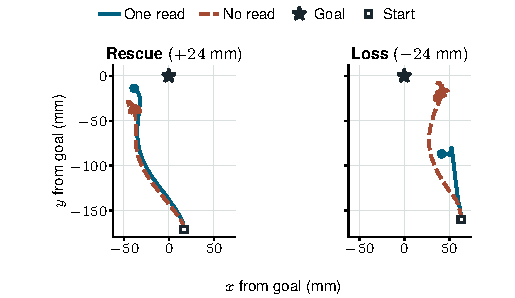
\includegraphics[width=\columnwidth]{figures/paired-push-paths.pdf}\par
{\footnotesize\sffamily
\makebox[.495\columnwidth]{No read, 44.2 mm}%
\makebox[.495\columnwidth]{One read, 96.2 mm}\par}

\includegraphics[width=\columnwidth]{figures/sawyer-push-terminal-views.pdf}\par
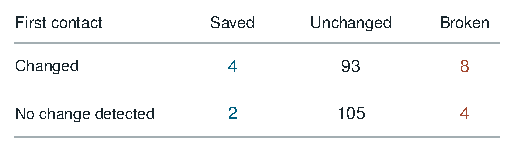
\includegraphics[trim=0 4bp 0 0,clip,width=\columnwidth]{figures/read-contact.pdf}
\caption{(Top) Object pushing trajectories in Sawyer layout 9123600 under $\pm 24\,\text{mm}$ initial object offsets, with dots marking final positions. This is the lowest-numbered layout exhibiting opposite outcome flips under mirrored offsets, shown at the shortest qualifying lead time (readback at step 36). (Middle) Matched camera views at the end of step 149 (0-indexed) for the negative-offset branches; the red cylinder is the object, the green sphere is the goal, and labels report final 3D distances from the simulator. (Bottom) Summary of first-contact changes and final outcomes across all 216 pairs; ``Saved'' denotes readback-only success and ``Broken'' denotes no-readback-only success.}
\label{fig:contact}
\end{figure}

Within the layout shown in Fig.~\ref{fig:contact}, every pair makes first contact on the same step, yet outcomes diverge sharply: under the $+24\,\text{mm}$ offset, readback reduces final 3D object-to-goal distance from $52.2\,\text{mm}$ to $41.1\,\text{mm}$, whereas under the $-24\,\text{mm}$ offset, it worsens the distance from $44.2\,\text{mm}$ to $96.2\,\text{mm}$. Across all 216 pairs, the median difference in the next written target is $6.40\,\text{mm}$. A total of 105 pairs exhibit at least one first-contact change: a change in whether a pad touches the object, a shift in the first-contact step, or at least a $2\,\text{mm}$ shift of the first-contact point in the object frame. Of these 105 pairs, 12 flip final outcomes; however, 6 of the remaining 111 pairs also flip outcomes. Detecting first-contact changes alone therefore misses some outcome-reversing cases.

Overall, the readback branch succeeds in 126/216 pairs versus 132/216 without readback, a difference of $-2.78$ percentage points (95\% layout-bootstrap CI: $[-5.56, -0.46]$). Before running the paired replays, we flagged queries that were within 5 steps of demonstrated contact and predicted at least a $1\,\text{mm}$ write difference from end-effector measurements. Of the 88 flagged pairs, 59 show first-contact changes, compared to 46 of the 128 unflagged pairs. Even when restricting attention to the 59 flagged pairs that also have nonzero object offsets, only 6 flip final outcomes, while 12 flips occur outside this subset.

\subsection{Selecting When to Read}

Using six development layouts, we selected and froze a state-based readback rule and evaluated it on 24 held-out Sawyer layouts. Each layout pairs the same three object positions with two input conditions (intact commands or five consecutive translational commands dropped), totaling 144 conditions. Within 18 steps before demonstrated contact, the rule may issue one query whenever end-effector deviation reaches $2.5\,\text{mm}$ and predicted target-write change reaches $1\,\text{mm}$. It has access to the demonstration, end-effector position, and command history, while object offsets and input faults remain hidden.

This state-based rule queries in all 72 dropped-input conditions and 4 of the 72 intact-command conditions. Its final outcome matches the no-readback observer and permuted-timing policy on every single pair (Fig.~\ref{fig:readbudget}). Compared with the paired fixed-timing policy---which reads one step before demonstrated contact, the best fixed step in development---the state rule saves one push and loses one, yielding a $0$ percentage-point difference (95\% layout-bootstrap CI: $[-2.08, 2.08]$). All six compared policies succeed in 75/144 pushes: 73 conditions succeed under all six policies, 67 fail under all six, and only 4 show any disagreement. Even an oracle selecting the best policy per condition post hoc could achieve at most 77/144.

\begin{figure}[t]
\centering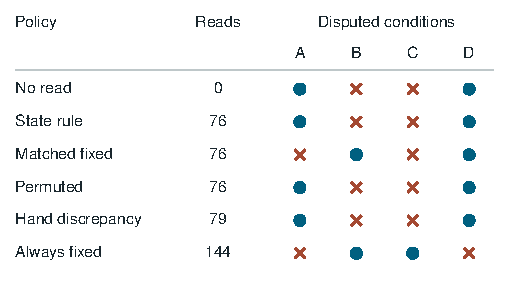
\includegraphics[trim=0 12bp 0 0,clip,width=\columnwidth]{figures/heldout-read-policy.pdf}
\caption{All four conditions out of the 144 held-out Sawyer pushing conditions where the six compared policies disagree on final success. Dots denote success and crosses denote failure. Layouts A--D are ordered by random seed; all involve dropped inputs with object offsets of $-24$, $+24$, $+24$, and $-24\,\text{mm}$, respectively. Read counts are totaled across all 144 pushes.}
\label{fig:readbudget}
\end{figure}

\subsection{Packet Delay and Target-Change Prediction}

On another 24 Sawyer layouts, we sample packets every three steps with a two-step delivery delay, carrying either three binary execution flags or the target at the sampling step. When commands are either passed intact or zeroed, both message types yield identical commands and end-effector trajectories across all 96 pairs. However, when five forwarded translational inputs are attenuated to one-quarter amplitude after the flag, mean end-effector RMS errors over 48 conditions are $10.126$, $5.149$, and $6.679\,\text{mm}$ for execution flags, target values, and empty packets, respectively (all completing 48/48 trials). Forwarding flags alone cannot verify the magnitude actually applied.

Assuming forwarded inputs are applied at full magnitude places the true origin outside the estimated box $\mathcal{B}$ in 5,025 of 7,200 attenuated steps, whereas allowing transmission gains between 25\% and 100\% covers all steps. Assuming the next command arrives intact, we also predict whether a readback will alter the written target by at least $1\,\text{mm}$. A shallow gradient-boosted tree classifier trained on eight layouts using origin bounds, sent commands, end-effector error, and received messages achieves 91.0\% balanced accuracy across 16 held-out layouts (43,200 correlated steps), compared to 85.8\% for a sent-command integration baseline; geometry alone resolves 2,861 of these steps with 100\% accuracy.



\section{Implications and Limitations}

Replay logs should record the command origin, command scale, initial target, and exact timing. For measured-origin controllers, end-effector measurements directly supply the origin; for accumulated-origin controllers, reconstructing the origin additionally requires knowing what inputs actually reached the target-writing function.

Our contact experiments rely on scripted pushing trajectories, synchronous readbacks, and known demonstration timing. Artificial object offsets and injected faults do not establish how often readbacks help in real-world deployment, and delayed packets describe stale states. Hardware validation will therefore require synchronized logging of applied low-level inputs, end-effector motion, and object contact.

\section{Conclusion}

Action limits govern how much correcting a command origin alters the next written target, while physical contact governs how that shift affects the manipulated object. In paired pushing trials, reading back the target can both rescue failing rollouts and break otherwise successful ones. Although end-effector motion and command history often expose dropped inputs, using them to schedule readbacks did not yield a net improvement in pushing success in our held-out timing experiments.

\section*{AI Tool Usage Disclosure}

OpenAI Codex assisted with experiment design, implementation, execution, literature verification, data analysis, plotting, and manuscript drafting.

\flushcolsend

\clearpage

\raggedcolsend

\begin{thebibliography}{8}

\bibitem{ref1}
Elie Aljalbout, Felix Frank, Maximilian Karl, and Patrick van der Smagt. On the role of the action space in robot manipulation learning and sim-to-real transfer. \emph{IEEE Robotics and Automation Letters}, 9: 5895--5902, 2024.

\bibitem{ref2}
Jiayuan Gu, Fanbo Xiang, Xuanlin Li, Zhan Ling, Xiqiang Liu, Tongzhou Mu, Yihe Tang, Stone Tao, Xinyue Wei, Yunchao Yao, Xiaodi Yuan, Pengwei Xie, Zhiao Huang, Rui Chen, and Hao Su. ManiSkill2: A unified benchmark for generalizable manipulation skills. In \emph{The Eleventh International Conference on Learning Representations}, 2023.

\bibitem{ref3}
Ajay Mandlekar, Soroush Nasiriany, Bowen Wen, Iretiayo Akinola, Yashraj Narang, Linxi Fan, Yuke Zhu, and Dieter Fox. MimicGen: A data generation system for scalable robot learning using human demonstrations. In \emph{Proceedings of the 7th Conference on Robot Learning}, volume 229 of \emph{Proceedings of Machine Learning Research}, pages 1820--1864, 2023.

\bibitem{ref4}
Matthias Plappert, Marcin Andrychowicz, Alex Ray, Bob McGrew, Bowen Baker, Glenn Powell, Jonas Schneider, Josh Tobin, Maciek Chociej, Peter Welinder, Vikash Kumar, and Wojciech Zaremba. Multi-goal reinforcement learning: Challenging robotics environments and request for research. \emph{arXiv:1802.09464}, 2018.

\bibitem{ref5}
Luca Schenato, Bruno Sinopoli, Massimo Franceschetti, Kameshwar Poolla, and S. Shankar Sastry. Foundations of control and estimation over lossy networks. \emph{Proceedings of the IEEE}, 95 (1): 163--187, 2007.

\bibitem{ref6}
Paulo Tabuada. Event-triggered real-time scheduling of stabilizing control tasks. \emph{IEEE Transactions on Automatic Control}, 52 (9): 1680--1685, 2007.

\bibitem{ref7}
Tianhe Yu, Deirdre Quillen, Zhanpeng He, Ryan Julian, Karol Hausman, Chelsea Finn, and Sergey Levine. Meta-World: A benchmark and evaluation for multi-task and meta reinforcement learning. In \emph{Proceedings of the Conference on Robot Learning}, volume 100 of \emph{Proceedings of Machine Learning Research}, pages 1094--1100, 2020.

\bibitem{ref8}
Yuke Zhu, Josiah Wong, Ajay Mandlekar, and Roberto Martín-Martín. robosuite: A modular simulation framework and benchmark for robot learning. \emph{arXiv:2009.12293}, 2020.

\end{thebibliography}



\end{document}
